\chapter{Preprocesado de datos}


Una vez examinados todos los conjuntos mencionados anteriormente, podemos llevar a cabo la unión de todos los datos en un único subconjunto. Esto nos permitirá conseguir un dataset completo y variado con diferentes tipos de piel y diferentes lesiones que nos permitirán identificar multitud de tipos de patologías, siendo posible ajustar el grado de granularidad en función de la agrupación o no de posibles subclases.

Inicialmente, el conjunto de datos construido contendrá todos los subtipos de lesiones cutáneas vistos, pero dispondrán de una segunda etiqueta que indicará si se trata de un caso canceroso o no, atendiendo a su subclase que lo etiqueta. Si agrupamos por lesiones benignas, cancerosas, y potencialmente cancerosas, podemos obtener el siguiente diagrama de sectores de la figura \ref{tartabinaria}, donde se puede observar cómo la mayoría de imágenes disponibles engloban problemas de piel no cancerosos, mientras que el segundo tipo más común de lesión si es la cancerosa. Si atendemos a clasificar las subclases de cada tipo de patología, encontramos 52 posibles etiquetas, las cuales iremos examinando a medida que se preprocese cada uno de los subconjuntos.


\begin{figure}[H]
	\centering
	\label {tartabinaria}
	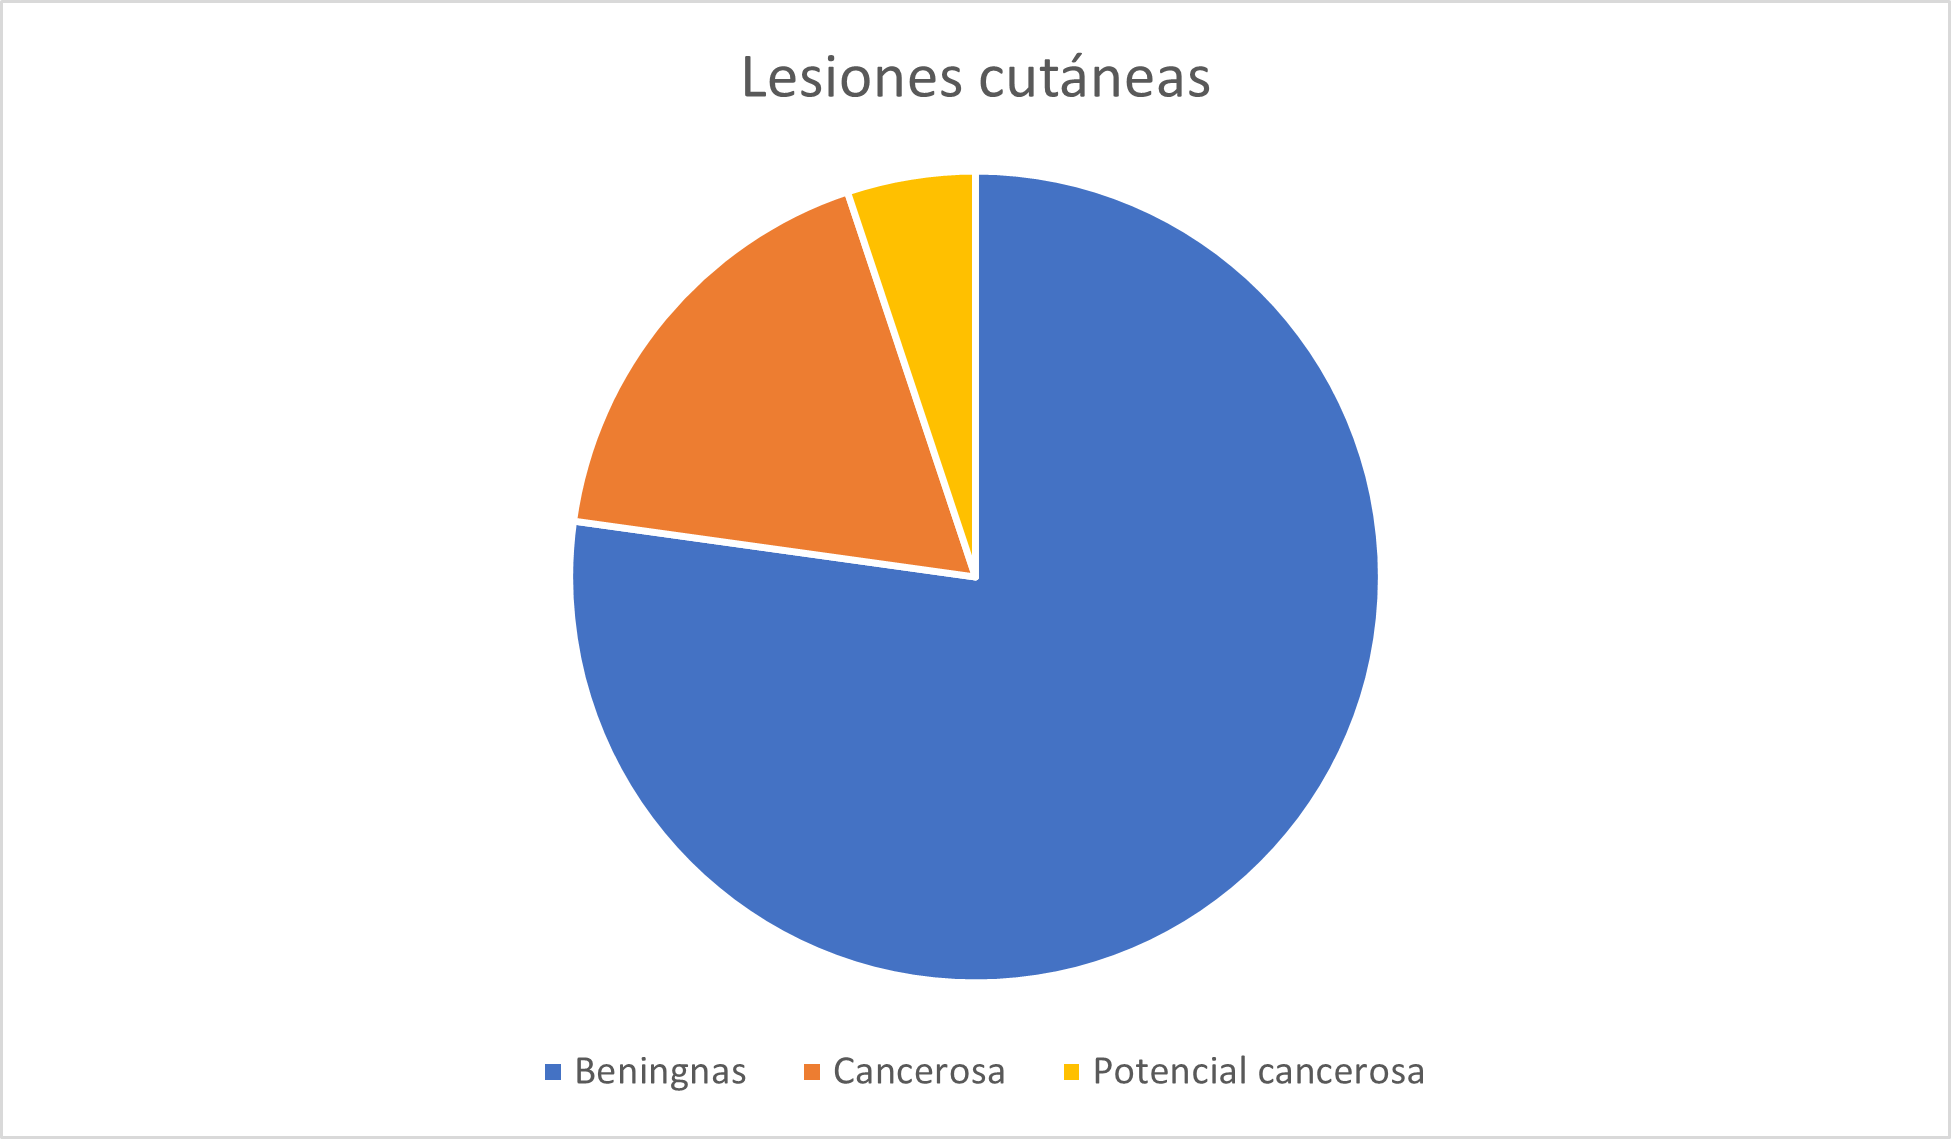
\includegraphics[scale = 0.7]{imagenes/datasetfinal.png}
	\caption{Distribución de clases}
\end{figure}

En el caso de las lesiones potencialmente cancerosas, como se trata de condiciones de la piel no cancerosas con posible evolución a cancerosas, se tendrán en cuenta como imágenes benignas, ya que la condición de malignidad sólo podría aparecer en el futuro, el cual sigue siendo desconocido.

El preprocesado de datos es una fase indispensable para el correcto aprendizaje de los algoritmos de deep learning. Se ha demostrado empíricamente que una correcta preparación y normalización de los datos permiten hallar soluciones más cercanas a la optima que con datos no procesados.

Es importante tener en cuenta que no existe una metodología de preprocesado única, y que es necesario adaptarse al tipo de dato que estamos tratando. Para este proyecto, además, existe una dificultad adicional, y es la existencia de diferentes procedencias para los datos, pues en total se dispone de 5 datasets distintos, cada uno recopilado con diferentes metodologías e instrumentación. Por tanto, será clave adaptarse a cada uno de los destinos, y realizar la partición final de forma estratificada para evitar sesgos que perturben el resutado.

a continuación, se describe la estrategia seguida para el procesado global de los datos, y los ajustes necesarios para cada uno de los conjuntos empleados.

\section{Estrategia de preprocesado para la fusión}

En el punto de partida, antes del preprocesado, contamos con 5 datasets muy diferentes entre sí. Cada uno ha sido documentado y organizado siguiendo unos criterios no estándares que nos afectan en gran medida a la hora de emplear estos datos para el aprendizaje. Antes de proceder con el desarrollo de los modelos, debemos de estadarizarlos a un formato común para evitar que existan clases con el mismo diagnóstico que, por cuestiones de formato, se consideren etiquetadas como clases distintas, por usar criterios distintos de escritura, como ausencia de espacio, mayúsculas o one hot encoding. 

Concretamente, los datos recopilados poseen el siguiente formato de etiquetado:
\begin{itemize}
	\item ISIC: etiquetas escritas a formato completo, como nombre de carpeta, con la primera letra de la enfermedad en mayúscula.
	\item ASAN: nombres escritos en el nombre de la fotografía, haciendo uso de caracteres especiales, y de abreviaturas.
	\item Severance: etiquetas escritas en la propia imagen, la cuales habrá que etiquetar y organizar manualmente, debido a que su csv está incompleto.
	\item PH2: fichero csv, con diagnósticos en formato one hot encoding. Es decir, una fila de ceros y unos, siendo uno la clase a la que pertenece, y 0, el resto.
	\item PAD UFES 20: fichero csv, con los nombres de diagnóstico escritos en minúsculas, sin espacios.
\end{itemize}

Podemos observar la gran variedad de formatos de registro empleados, y que por tanto, es completamente obligatorio y necesario realizar una transformación para hacerlo homogéneo. En este caso, por decisión propia, he considerado adecuado realizar una transformación de las etiquetas al siguiente formato: Uso únicamente de minúsculas, con ausencia de caracteres especiales, nombres sin abreviaturas, y evitando el uso de espacios, con el uso de la barra baja como carácter sustitutivo. Para la clasificación binaria, se utilizará one hot encoding, denotando como 0 los casos negativos y como unos, los positivos.\\


De esta forma, se obtiene un fichero .csv donde encontrar los valores necesarios para entrenar los modelos. Para poder localizar cada imagen, se mantendrá el arbol de directorios por defecto de cada dataset, y se anotará su directorio en un nuevo fichero .csv, que contendrá las etiquetas estandarizadas y los nombres de los ficheros de imagen con y sin el directorio. En resumen, contará con los campos:

\begin{itemize}
	\item image: nombre la imagen, sin el path en su nombre, y con la extensión de formato
	\item dir: directorio donde se aloja la imagen, respetando la estructura de carpetas original seguida por el dataset de origen
	\item label: etiqueta con el diagnóstico de la lesión, siguiendo las pautas indicadas anteriormente
	\item dataset: columna que indica el dataset de procedencia de la imagen, por si fuese necesario utilizar solo un subconjunto de todos los datos.
	\item bin: columna para la etiqueta que indica si se trata de clase Benigna (0) o Maligna (1)
\end{itemize}

\begin{figure}[H]
	\centering
	\label {formatocsv}
	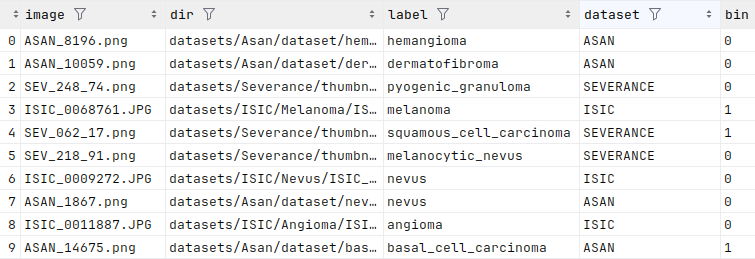
\includegraphics[scale = 0.55]{imagenes/formatocsv.png}
	\caption{Formato del fichero csv normalizado}
\end{figure}

Una vez establecido el formato común, podemos pasar al análisis y adaptación propia de cada conjunto.

\subsection{ISIC Dataset}

El dataset ISIC es el mayoritario de la lista, ya que posee casi 60.000 imágenes de alta resolución, del total de casi 108.000 imágenes de las que disponemos. Para su descarga, se han empleado la galería de la web oficial \cite{isicarchive}, donde podemos filtrar cómodamente las enfermedades que queremos descargar. Como criterio de descarga, se han tenido en cuenta únicamente aquellas fotografías correctamente diagnosticadas, ya que existe un total de 27896 imágenesno etiquetadas dentro del repositiorio, las cuales descartaremos. El problema se centrará en resolver un problema de aprendizaje supervisado, por lo que las imágenes no etiquetadas suponen una complejidad adicional y un ruido para el modelo.

Cada clase descargada, además, se ha sometido a un proceso de filtro, sobre todo por cuestiones numéricas; existen nuevas clases, con escasas cantidades de datos, las cuales poseen menos de 10 imágenes, cantidad insuficiente a la hora de clasificar frente a clases como lunares comunes, que tienen en total 32697 ejemplares. De esta forma, nos queda el siguiente conjunto de clases:
\begin{itemize}
	\item Nevus
	\item Seborreic keratosis            
	 \item Actinic keratosis            
	\item Pigmented benign keratosis         
	\item Solar lentigo                           
	\item Dermatofibroma                          
	\item Vascular lesion                         
	\item LIchenoid keratosis                     
	\item Acrochordon                             
	\item Lentigo NOS                             
	\item Atypical melanocytic proliferation       
	\item Aimp                                     
	\item 	Wart                                     
	\item Angioma                                  
	\item Lentigo simplex                          
	\item 	Neurofibroma                             
	 \item 	Scar 
\end{itemize}

Estas clases se almacenan en ficheros zip cada una, así que tras ser descargadas, deben ser extraídas y añadidas al fichero csv que definimos anteriormente. Al tratarase del primer subconjunto que se añadirá, será la parte del código encargada de crear el fichero y establecer las columnas mencionadas. Además, se realizará la transformación de las etiquetas, dispuestas en el formato de la enumeración anterior, a notación snake case. Numerando el proceso, se ha creado un script de python que realiza las siguientes tareas:

 
 \begin{algorithm}[H]
 	\label{extract}
 	\caption{Algoritmo de descompresión de fotografías por carpetas}
 	\begin{algorithmic}[1]
 		
 		\Procedure{extractISIC}{path}
 		\Comment{Obtener una lista de todos los archivos ZIP}
 		 		\State archivosZip : list of strings
 		 		
 		\ForAll{file in path where file.name endswith('zip')}
 			\State archivosZip.add(file)
 		\EndFor

		\Comment{Iterar sobre cada archivo ZIP}
			\ForAll{archivo in archivosZip}
			\State var rutaArchivoZip  $\gets$ join(path, archivo)
			\State var carpetaSalida = path.splitext(rutaArchivoZip).get(0) \Comment{ Eliminar la extensión}
		
			\If {not exists(carpetaSalida)}
				\State makedir(carpetaSalida) 

			\Comment{  Extraer el contenido del archivo ZIP en la carpeta de salida}
			\State \Call{openZipFile}{rutaArchivoZip} as zipRef
			\State zipRef.extractall(carpetaSalida)
			 \EndIf
		\EndFor
 		\EndProcedure
 		
 	\end{algorithmic}
 \end{algorithm}
 
 


\begin{enumerate}
	\item Extraer las imágenes mediante uzip en una carpeta con el mismo nombre de la clase a la que pertenecen \ref{extract}
	\item Crear un fichero .csv, denominado preprocessedData.csv, donde se alojarán las 5 columnas: images, dir, label, dataset, bin.
	\item Recorrer cada carpeta creada, y añadir los 4 primeros campos
	\item Una vez añadidas todas las imágenes, se renombran las etiquetas a camel case mediante las funciones upper(), lower() y replace() de la clase string de python.
\end{enumerate}

\begin{algorithm}[H]
		 \label{isiccrear}
		\caption{Algoritmo de creación del csv}
		\begin{algorithmic}[1]
			
		\Procedure{crear\_csv}{path, clases, nombre\_dataset}
		\Comment {Inicializa una lista vacía para almacenar la información de los archivos}
		 \State var info\_archivos : list of strings
		 \State i  $\gets$ 0
		
		 \For{nombre\_carpeta in dir(path)}
			\State ruta\_carpeta $\gets$join(path, nombre\_carpeta)
			
			\If{path.isdir(ruta\_carpeta)}
		
				\Comment {Itera sobre cada archivo en la carpeta}
				\For{nombre\_archivo in listdir(ruta\_carpeta)}
						  \State ruta\_archivo $\gets$ join(ruta\_carpeta, nombre\_archivo)
					\If {isfile(ruta\_archivo) and nombre\_archivo.ends() != "jpg"}
						\State var info\_archivos.add(nombre\_archivo, ruta\_archivo, clases[i], nombre\_dataset)
					\EndIf
					\State i = i + 1
				\EndFor
		 	\EndIf
		\EndFor		
		
	
		\State ruta\_archivo\_csv $\gets$ 'preprocessedData.csv'	\Comment{ Define la ruta del CSV}
		
		\State open(ruta\_archivo\_csv) as archivo\_csv
		 \State archivo\_csv.writerow(["image", "dir", "class", "dataset"])  
		 \Comment{Escribe la cabecera}
		 
		 \EndProcedure
	\end{algorithmic}
\end{algorithm}

Para facilitar el procesado, el rellenado de los datos se realiza sobre una estructura tabular de pandas, para así transformar la columna label fácilmente.
En cuanto a la quinta columna, la clase binaria, dicha tarea se realizará cuando todos los datasets estén añadidos al .csv, de forma que el recorrido de los datos sólo se realice una vez, cuando tengamos disponible todas las clases. 

En cuanto al estudio estadístico de los datos, este se realizará una vez dividido los datos en los conjuntos de entrenamiento y test, definido en entradas posteriores.

\subsection{ASAN}

ASAN es uno de los dos datasets cuyo formato de entrega de los datos consistía en una matriz de imágenes en un canvas de gran resolución. En el caso de este dataset, tenemos un total de 32 imágenes de este tipo, cuya etiqueta se encuentra escrita en el nombre del fichero.
El procesado de este dataset será más complejo que el anterior, ya que debemos recortar cada una de las imágenes, evitando que queden bordes blancos que puedan perturbar la predicción, y sesgar el aprendizaje.

Podríamos idear una solución codificada de forma estricta en la cual la imagen se subdivida en n filas y m columnas para extraer las fotografías; sin embargo, cada uno de los canvas del datasets tiene un número filas y columnas concreto que dificultaría esta tarea de forma automática. En su lugar, se ha medido mediante una herramienta de recorte fotográfico el tamaño de una de las miniaturas, siendo este de 98 píxeles, y será el valor que utilizaremos a la hora de realizar el recortado.

No se debe pasar por alto que las imágenes se encuentran separadas vertical y horizontalmente por espacios en blanco, cuya distancia es variable. Es el factor causante de la imposibilidad de partición regular, por lo que se emplearán técnicas de visión mediante la librería OpenCV para la detección de bordes:

\begin{enumerate}
	\item Eliminar 4 píxeles en blanco de los extremos para que todas las bandas blancas queden del mismo grosor
	\item Hallar el numero de imágenes por fila y columana de forma aproximada, teniendo en cuenta el tamaño de miniatura y el borde.
	\item Recortar la imagen usando el método findContours() de openCV. Este método binaria la imagen transformándola a blanco y negro, y trazado con técnicas de detección de puntos de interés en imágenes los bordes de cada una de las miniaturas, y devolviendo las coordenadas de sus equinas en un vector multidimensional. 
	\item Para cada imagen, obtenemos la esquina superior izquierda de la imagen, y mediante el ancho y alto de la imagen, recortamos dicha sección de la imagen y se almacena en una nueva variable.
	\item Se recortan los bordes de dicha imagen y se almacena el resultado en disco, en una carpeta que posee el mismo nombre que la imagen de la que fue extraída.
	\item Se repite el paso 3-6 para cada imagen de la matriz, pasando a abrir la siguiente matriz hasta que no quede ninguna por recortar.
\end{enumerate}

\begin{algorithm}[H]
		\label{cortarasan}
		\caption{Recorte de las imágenes de ASAN mediante OpenCV}
		\begin{algorithmic}
			\Procedure{recortarImagenesASAN}{path, i, title='ASAN'}
			\State var files : list of strings
			
			 \For {f in pathlib.Path().iterdir()}
			 	 \If {f is\_file()]}
			 	 	\State files.add(f)
			 	 \EndIf
			 \EndFor
			 	 
			\State var names : list of strings
			\State var  diss\_class : list of strings
			 \State var i $\gets 0$
			
			\ForEach {f in files}
				   \State name $\gets$ str(f)[str(f).rfind('\#') + 1:-4]
				   \If {f.ends = 'png' and not exists(path)}
						\State {makedir(name)}
						\State var image = cv2.imread(str(f), cv2.IMREAD\_UNCHANGED): image
						\State var gray = cv2.cvtColor(image, cv2.COLOR\_BGR2GRAY) : image
			
						\State var kernel = cv2.getStructuringElement(cv2.MORP H\_RECT, (5, 5))
						\State var gradient = cv2.morphologyEx(gray, cv2.MORPH\_GRADIENT, kernel)
			
						\State var contours $\gets$ cv2.findContours(gradient, cv2.RETR\_EXTERNAL, cv2.CHAIN\_APPROX\_SIMPLE)
			
						\ForEach{cnt in contours}
								\State	x, y, w, h  $\gets$ cv2.boundingRect(cnt)
								\State var box\_image = image[y: y + h, x: x + w] : image
				
								 \Comment{Recorta la imagen para eliminar el borde} 
								\State var img\_sin\_borde = box\_image[grosor\_borde:-grosor\_borde, grosor\_borde:-grosor\_borde]
								\State cv2.imwrite(f"{name}/{title}\_{i}.png", img\_sin\_borde)
					
								\State names.append(f"{title}\_{i}.png")
								\State diss\_class.add(name)
								
								\State i = i + 1
						 \EndFor
				\EndIf	 
	\EndFor
				
\EndProcedure
\end{algorithmic}
\end{algorithm}

Una vez finalizado el proceso, el proceso a aplicar es similar a ISIC; pero, en este caso, en lugar de simplemente convertir a camelcase, debemos de cambiar los nombres por completo para no usar el formato por abreviaturas original, y poder hacer merge de las clases de este dataset con ISIC que sean de la misma enfermedad. Para ello, simplemente se crea un diccionario clave-valor, donde la clave es el nombre que deseamos cambiar, y el valor, el nuevo nombre. Mediante pandas, el proceso de sustitución se puede hacer de forma inmediata mediante la función replace.

Es importante destacar que el dataset Hallym, también será incluido en el conjunto final, siendo el procedimiento de preprocesado a aplicar exactamente el mismo al descrito en este punto.

\subsection{PAD UFES 20}

PAD UFES 20, como ya describimos en el apartado de Estado del arte, se trata de un dataset diseñado para el entramiento de sistemas de asistencia en diagnóstico computado, donde el experto dermatólogo puede utilizarlo como un medio de apoyo. Contiene 6 enfermedades distintas, siendo 3 cancerosas (células basales, células escamosas o melanoma maligno) y 3 benignas (actinic keratosis, nevus, keratosis seborreica).

La estructura de presentación de los datos es más sencilla que ASAN, pues las imágenes son individuales, y cuentan con un fichero .csv donde se describen las etiquetas y otros metadatos asociados a las imágenes. La única modificación necesaria es actualizar el path de cada imagen y la nomenclatura del diagnóstico de la enfermedad, teniendo en cuenta que debemos de tranformar de abreveviatura a camel case:
\begin{itemize}
	\item NEV $\rightarrow$ nevus
	\item SEK  $\rightarrow$ seborreic\_keratosis 
	\item ACK $\rightarrow$ actinic\_keratosis  
	\item BCC $\rightarrow$  basal\_cell\_carcinoma           
	\item SCC $\rightarrow$ squamous\_cell\_carcinoma
	\item MEL $\rightarrow$ melanoma
	         
\end{itemize}



\begin{algorithm}
	\label{cortarpadufes}
	\caption{Formato de las imágenes de PAD UFES}
	\begin{algorithmic}
		\State  var PAD\_UFES\_PATH : directory of PAD UFES 20 dataset
		\State dict $\gets$ \{'BCC': 'basal\_cell\_carcinoma', 'SEK': 'seborreic\_keratosis', 'SCC': 'squamous\_cell\_carcinoma', 'NEV': 'nevus',
			'ACK': 'actinic\_keratosis', 'MEL': 'melanoma'\}
		\Procedure{preparar\_padufes}{}
		\State df\_pad\_ufes $\gets$ file.read()
		\State  df\_pad\_ufes['diagnostic'] $\gets$ df\_pad\_ufes['diagnostic'].replace(dict)
		
		\ForEach{img in df\_pad\_ufes}
			\State df\_pad\_ufes['im\_dir'] $\gets$  PAD\_UFES\_PATH + '/images/ + img
		   \State df\_pad\_ufes['dataset'] = 'PAD\_UFES'
	
	\EndFor		
		\EndProcedure
	\end{algorithmic}
\end{algorithm}

De esta forma, podemos simplemente hacer fusión de las nuevas filas con el fichero anterior en modo de apertura ``append''.

\subsection{PH2}

Este dataset recoge imágenes provenientes del Servicio de Dermatología del Hospital Pedro Hispano (Matosinhos, Portugal), que recoge pruebas cutáneas realizadas con el sistema Tuebinger Mole Analyzer, y un aumento de 20x. Recordando lo analizado en el capítulo anterior, consta de 200 imágenes dermatoscópicas de lesiones melanocíticas, incluidos 80 lunares comunes, 80 nevus atípicos y 40 melanomas, en una resolución de 768x560 píxeles. La base de datos PH² incluye anotaciones médicas de todas las imágenes: segmentación médica de la lesión, diagnóstico clínico e histológico, y evaluación de varios criterios dermatoscópicos. Entre ellos, encontramos distinción por colores; formación del tejido; puntos/glóbulos; rayas; áreas de regresión; velo azul blanquecino (pgimentación difusa).

Los datos se organizan en directorios de carpetas de varios niveles,  pudiendo encontrar en su interior la imagen dermoscópica, la plantilla de segmentación y regiones de interés de la imagen destacadas mediante una plantilla binaria. Para este trabajo, sólo se utilizarán las imágenes correspondientes al directorio de datos dermoscópicos, ya que con debido a la cercanía de la lensión, la imagen contiene en su mayoría solo información útil.

Como preprocesado de las imágenes, al disponer de ellas correctamente clasificadas en carpetas y con un fichero de metadatos bastante completo, el único procedimiento necesario sería la adición al fichero preprocessedData.csv, realizando las conversión a camel case de las labels. El método a emplear es equivalante al utilizado en PAD UFES \ref{cortarpadufes}.

 \subsection{Severance}
 
 Este dataset, como ya se comentó, provinene del hospital Severance, y el dataset con mayor cantidad de patologías identificadas de la lista. El formato de este repositorio sigue una estructura similar a la de ASAN: las imágenes están organizadas en varias páginas de gran tamaño, donde, a diferencia de ASAN, podemos encontrar varias imágenes por lesión separadas entre cuadros blancos, que contienen escritos en él, la etiqueta de las siguientes imágenes leídas de izquierda a derecha, y de arriba a abajo, hasta encontrar el siguiente cuadro en blanco con texto.
 
 La dificultad de este preprocesado radica precisamente en la existencia de los cuadrados blancos, ya que la lectura del texto escrito en ellos es prácticamente imposible. La baja resolución, unido a la existencia de etiquetas cuyo nombre se encuentra dividido en varias líneas, provoca que algoritmos de reconocimiento de texto como Pytesseract \cite {pytesseract} no fuesen capaces de detectar las etiquetas adecuadamente.
 
 Por este motivo, fue necesario identificar manualmente cuántos casos de cada enfermedad existían por matriz de imágenes, y realizar un recuento para saber cuándo aplicar una etiqueta u otra. Conociendo que las etiquetas asignadas aparecían por orden alfabético, el proceso a seguir se resumió en aumentar un contador cada vez que aparecía una imagen en blanco durante el recorrido de las imágenes, y aumentar el contador hasta llegar al valor total de ejemplares de esa clase; en ese momento, se procede a contar los valores de la siguiente. Con este procedimiento, nos queda el algoritmo \ref{cortarseverance}
  
La ventaja respecto a ASAN reside en que los espacios en blanco entre imágenes tienen el mismo grosor, y fue posible de separar en submatrices sin necesidad de utilizar ténicas de visión, que ralentizan el proceso extracción. Cada imagen es etiquetada siguiendo el formato establecido  y siendo añadida a una nueva carpeta, desde la cual se referenciarán mediante el fichero preprocessedData.csv. 

Como dificultades a destacar durante el desarrollo de este procedimiento, comentar que la detección de la imagen en blanco que separa las etiquetas entre clases no es trivial. El método elegido para distinguirla es emplear un  umbral de número de píxeles con valor de escala de grises blanco, es decir, 255. El valor de dicho umbral se calculó de forma experimental , ya que si el valor era demasiado bajo, pieles sanas o de color claro también cumplían la restricción. El cambio de etiquetado no se produce si el número de píxeles totales de la imagen encontrada no supera un valor x de miles de píxeles. De forma experimental, el valor 20.000 fue el que mejor resultados aportó, funcionando en todos los casos.

Aumentar de forma desmesurada este valor también puede tener consecuencias negativas, ya que el nombre de la etiqueta se encuentra escrita en la parte inferior de estas imágenes y aportan píxeles de color negro que no cumplirían la condición.


 \begin{algorithm}[!ht]
	\label{cortarseverance}
	\caption{Recorte de las imágenes de Severance mediante OpenCV}
	\begin{algorithmic}
		\Procedure{recortarImagenesSEVERANCE}{path}
		
		\State  df\_sev $\gets$ read('SeveranceA.xls')
		\If {not os.path.exists('thumbnails')}
		\State makedir('thumbnails')
		\EndIf
		
		\State var files : list of strings
		
		\For {f in pathlib.Path().iterdir()}
		\If {f is\_file()]}
		\State files.add(f)
		\EndIf
		\EndFor
		
		\State var names : list of strings
		\State diss\_class : list of strings
		\State j $\gets 0$
		
		\For {f in files}
		\If {f.ends = 'jpg'}
		\State name $\gets$ f.name[0:-4]
		\State {makedir(name)}
		\State var image = cv2.imread(name, cv2.IMREAD\_UNCHANGED): image
		\State var image\_split = $\begin{matrix}
			[ image_1 image_2, \ldots, image_8 ] \end{matrix}^T$	\Comment{División por filas}
		
		
		\State var i $\gets$ 0
		
		\ForEach{im  in image\_split}
		\Comment{Recorta la imagen en columnas}
		\State image\_split\_col = np.split(im[:, 2:-3], 15, axis=1)
		\ForEach {imcol in image\_split\_col}
		\State img\_sin\_borde$\gets$ imcol[grosor\_borde:-grosor\_borde, grosor\_borde:-grosor\_borde]
		\If {np.count\_nonzero(imcol == 255) > 20000)}  \Comment{Si es imagen de separador con nombre}
		\State j $\gets j + 1$  \Comment {Cambiamos de etiqueta al siguiente paciente}
		\State continue
		\Else
		\State actual  $\gets$ df\_sev.get(j)
		
		\State	actual.add('{name}\_{i}.png')
		\State	trainProcessed.add(actual)
		\Comment{Guardamos la imagen y añadimos su nombre}
		\EndIf
		\State cv2.imwrite(f'thumbnails/{name}\_{i}.png', img\_sin\_borde)
		\State names.append(f"{name}\_{i}.png")
		\State i $\gets i + 1 $
		
		\State diss\_class.add(name)
		\EndFor
		
		\EndFor
		\EndIf	 
		\EndFor
		\State trainProcessedDF.write("severanceTrainingSet\_thumbnails.csv") \Comment{Guardado en disco}
		\EndProcedure
	\end{algorithmic}
\end{algorithm}
 
 \section{Etiquetado binario}
 
 Tras la homogeneización de los datos de todos los conjuntos, debemos realizar el etiquetado binario de las imágenes. En lugar de realizar este proceso durante la adaptación de los datos, se decidido realizar este procedimiento una vez el fichero csv estuviese completamente convertido, de forma que el recorrido de los datos es mucho más sencillo al ser completamente lineal. Para ello, simplemente se ha creado una nueva columna mediante el uso de pandas que recibe como parámetro una diccionario con las etiquetas totales del dataset, 54.  Este diccionario, realizado manualmente, contiene un 0 en aquellas clases correspondientes a lesiones benignas de la piel, mientras que el 1 quedo reservado para aquellas lesiones malignas que son cancerosas.
 
 Gracias a la función replace el proceso consiste ;
 
 \begin{enumerate}
 	\item Clonar la columna target, que contiene las etiquetas multiclase
 	\item Aplicar la función replace() de pandas, que recibe como argumento el diccionario confeccionado para la sustitución.
\end{enumerate}

De esta forma, obtenemos la quinta columna, y podemos dar por finalizado la primera fase del preprocesado de datos.